\documentclass{beamer}
\usepackage{graphicx}
\usepackage{amsmath}

\title{Evolución del Potencial de Weyl \\ y Discrepancias con $\Lambda$CDM}
\author{Manuel Garcia}
\date{\today}

\begin{document}

\frame{\titlepage}

\section{Introducción}


\begin{frame}
\frametitle{¿Qué es el potencial de Weyl?}
\begin{itemize}
    \item Combina las perturbaciones espaciales (\( \Phi \)) y temporales (\( \Psi \)) del universo:
    \[
    \Psi_W = \frac{\Phi + \Psi}{2}
    \]
    \item Proporciona una forma directa de probar:
    \begin{itemize}
        \item La validez de la Relatividad General (GR).
        \item El modelo estándar cosmológico (\( \Lambda\text{CDM} \)).
    \end{itemize}
    \item Es medido usando datos de lentes gravitacionales y clustering de galaxias.
\end{itemize}
\end{frame}

\section{Problemas observados}

\begin{frame}
\frametitle{Discrepancias observadas}
\begin{itemize}
    \item Las mediciones del potencial de Weyl en el Dark Energy Survey (DES) muestran:
    \begin{itemize}
        \item Valores por debajo de las predicciones de \( \Lambda\text{CDM} \) en los primeros dos intervalos de redshift.
        \item Una tensión de \( 2\sigma \) y \( 2.8\sigma \) en \( z = 0.295 \) y \( z = 0.467 \), respectivamente.
    \end{itemize}
    \item Esto podría deberse a:
    \begin{itemize}
        \item Modificaciones a GR.
        \item Errores en el modelado no lineal.
    \end{itemize}
\end{itemize}
\begin{figure}
    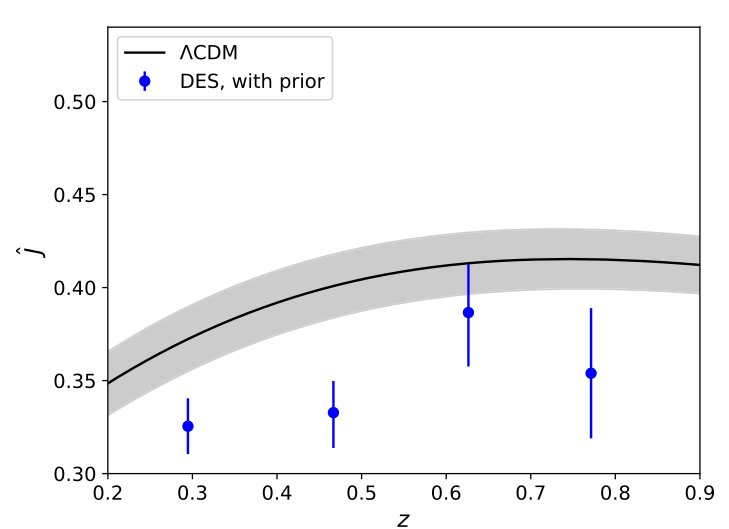
\includegraphics[width=0.5\textwidth]{CMB_weyl.png} 
    \caption{Mediciones de \( J(z) \) utilizando información de CMB.}
\end{figure}
\end{frame}

\section{Metodología}

\begin{frame}
\frametitle{Mediciones independientes de modelos}
\begin{itemize}
    \item Método que mide directamente \( J(z) \):
    \[
    J(z) = \frac{\Psi_W}{\sigma_8(z)}
    \]
    \item Combina observaciones de:
    \begin{itemize}
        \item Lentes gravitacionales de galaxias.
        \item Clustering de galaxias.
    \end{itemize}
    \item No asume teorías específicas de gravedad.
\end{itemize}
\begin{figure}
    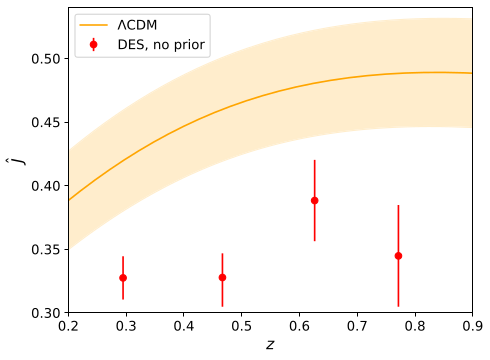
\includegraphics[width=0.5\textwidth]{noCMB_weyl.png}
    \caption{Mediciones de \( J(z) \) sin utilizar información de CMB.}
\end{figure}
\end{frame}

\section{Resultados y discusiones}

\begin{frame}
\frametitle{Resultados principales}
\begin{itemize}
    \item El potencial de Weyl muestra un crecimiento más lento a bajas redshifts.
    \item Las discrepancias persisten incluso sin usar información del CMB.
    \item Se observan indicios de que GR podría no ser válida en todas las escalas.
\end{itemize}
\begin{figure}
    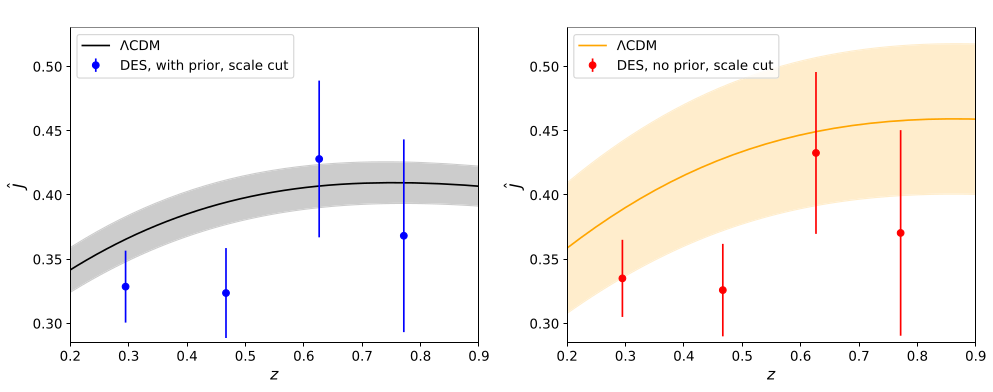
\includegraphics[width=0.9\textwidth]{scale_cut_CMB_weyl.png} 
    \caption{Comparación de \( J(z) \) con predicciones de $\Lambda$CDM usando cortes en la escala.}
\end{figure}
\end{frame}

\section{Implicaciones y futuro}

\begin{frame}
\frametitle{Implicaciones y próximos pasos}
\begin{itemize}
    \item Modelos gravitatorios modificados:
    \begin{itemize}
        \item Teorías de Horndeski.
        \item Extensiones fenomenológicas (\( \mu, \Sigma \)).
    \end{itemize}
    \item Próximos experimentos como \textbf{Euclid} y \textbf{LSST}:
    \begin{itemize}
        \item Reducirán las incertidumbres en \( J(z) \).
        \item Ampliarán el rango de redshifts observables.
    \end{itemize}
\end{itemize}
\end{frame}

\begin{frame}[allowframebreaks]
\frametitle{Referencias}

\begin{thebibliography}{99}

\bibitem{paper-original}
Tutusaus, I., Bonvin, C., Grimm, N. (2024). \textit{Measurement of the Weyl potential evolution from the first three years of Dark Energy Survey data}. Nature Communications, 15, 9295. \url{https://doi.org/10.1038/s41467-024-53363-6}.

\bibitem{news}
Phys.org. (2024, Noviembre). \textit{Theory team investigates Einstein's distortion of space}. \url{https://phys.org/news/2024-11-theory-team-einstein-distortion-space.html}.

\end{thebibliography}

\end{frame}

\end{document}
